\documentclass[lettersize,journal]{IEEEtran}
\usepackage{amsmath,amsfonts}
\usepackage{algorithmic}
\usepackage{array}
\usepackage{textcomp}
\usepackage{stfloats}
\usepackage{url}
\usepackage{verbatim}
\usepackage{graphicx}
\usepackage{algorithm}
\usepackage{array}
\usepackage{cite}
\usepackage{subfigure}
\usepackage{kotex}
\usepackage{bbm}
\usepackage{hyperref}
\usepackage{xcolor} % 삭제 예정
\newcommand{\tred}{\textcolor{red}}

\hyphenation{op-tical net-works semi-conduc-tor IEEE-Xplore}
\def\BibTeX{{\rm B\kern-.05em{\sc i\kern-.025em b}\kern-.08em
    T\kern-.1667em\lower.7ex\hbox{E}\kern-.125emX}}

\newcolumntype{M}[1]{>{\centering\arraybackslash}m{#1}}
\usepackage{balance}
\begin{document}
\title{Novel Channel Estimation Based on Enhanced Diffusion Posterior Sampling for mmWave Massive MIMO Systems}

\author{\IEEEauthorblockN{Jinwook Kim,~\IEEEmembership{Graduate Student Member,~IEEE}},  \IEEEauthorblockN{Seongwoo Lee,~\IEEEmembership{Graduate Student Member,~IEEE}},

\IEEEauthorblockN{Soo Hyun Kim,~\IEEEmembership{Member,~IEEE}}, \IEEEauthorblockN{Young Ghyu Sun,~\IEEEmembership{Member,~IEEE}},
\IEEEauthorblockN{Joonho Seon,~\IEEEmembership{Graduate Student Member,~IEEE}},

\IEEEauthorblockN{Hyowoon Seo,~\IEEEmembership{Member,~IEEE}}, \IEEEauthorblockN{Dong In Kim,~\IEEEmembership{Life Fellow,~IEEE}}, and \IEEEauthorblockN{Jin Young Kim,~\IEEEmembership{Senior Member,~IEEE}
\vspace{-10pt}
}
        % <-this % stops a space
% \thanks{This work was 
% partly supported by Institute of Information \& communications Technology Planning \& Evaluation (IITP) grant funded by the Korea government (MSIT) (No. 2021-0-00892-005, Research on advanced physical layer technologies of low-earth orbit (LEO) satellite communication systems for ubiquitous intelligence in space) and 
% supported by the MSIT(Ministry of Science and ICT), Korea, under the ITRC(Information Technology Research Center) support program(IITP-2025-RS-2023-00258639) supervised by the IITP(Institute for Information \& Communications Technology Planning \& Evaluation).}% <-this % stops a space
\thanks{Jinwook Kim, Seongwoo Lee, Soo Hyun Kim, Young Ghyu Sun, Joonho Seon, and Jin Young Kim are with the Department of Electronic Convergence Engineering, Kwangwoon University, Seoul 01897, South Korea (e-mail: \{yoonlight12, swoo1467, kimsoogus, yakrkr, dimlight13, jinyoung\}@kw.ac.kr).}
\thanks{Hyowoon Seo, and Dong In Kim are with the Department of Electrical and Computer Engineering, Sungkyunkwan University, Suwon 16419, South Korea (e-mail: \{hyowoonseo,dongin\}@skku.edu).}}


% The paper headers
\markboth{IEEE communications letters, ~Vol.~15, No.~8, August~2025}%
{Shell \MakeLowercase{\textit{et al.}}: A Sample Article Using IEEEtran.cls for IEEE Journals}

\maketitle
\begin{abstract}
In this letter, a novel channel estimation method based on diffusion posterior sampling is proposed for effective millimeter-wave (mmWave) massive multiple-input multiple-output (MIMO) systems to address the trade-off between accuracy, pilot overhead, and complexity. The proposed method is derived by approximating the likelihood score using moment matching and Tweedie's formula to enable accurate and efficient posterior sampling. From the simulation results, the proposed method outperforms the baselines in terms of estimation accuracy, while achieving a comparable computational complexity to the state-of-the-art diffusion model-based channel estimation methods under low pilot overhead in both line-of-sight and non-line-of-sight environments.
\end{abstract}

\begin{IEEEkeywords}
Channel estimation, mmWave, massive MIMO, diffusion model, moment matching, Tweedie's formula.
\end{IEEEkeywords}


\section{Introduction}

In modern wireless communication systems, millimeter-wave (mmWave) massive multiple-input multiple-output (MIMO) has emerged as a key technology, which can provide significant advantages in data rates and spectral efficiency. To realize these advantages, the accurate acquisition of channel state information through channel estimation is required~\cite{busariMillimeterWaveMassiveMIMO2018}. Traditional channel estimation approaches, including least squares (LS) and minimum mean squared error (MMSE), have been widely used owing to their simplicity and well-established theoretical foundations. Nonetheless, these methods are often constrained by performance degradation, reduced spectral efficiency, and excessive pilot overhead, primarily due to the high dimensionality introduced by the large number of antennas~\cite{hassibiHowMuchTraining2003}. While compressed sensing (CS)-based approaches can significantly reduce pilot overhead by leveraging the inherent sparsity of mmWave channels, their performance is highly sensitive to the accuracy of the sparsity and channel modeling~\cite{zhangAtomicNormDenoisingBased2018,mendez-rialHybridMIMOArchitectures2016,choiCompressedSensingWireless2017}.

These limitations have motivated research into deep learning (DL)-based channel estimation, which has been confirmed to have better approximation capability~\cite{kimDeepLearningaidedWireless2023, heDeepLearningBasedChannel2018}. In particular, diffusion models (DMs), well-known generative models, have attracted considerable attention for their ability to approximate complex data distributions~\cite{arvinteMIMOChannelEstimation2023,feslDiffusionBasedGenerativePrior2024,zhouGenerativeDiffusionModels2025}. The DM-based posterior sampling method for channel estimation has been introduced in~\cite{arvinteMIMOChannelEstimation2023}, demonstrating superior estimation accuracy compared to state-of-the-art methods. However, a large number of sampling steps are required to achieve this performance. To address this limitation, a denoising strategy for the DM-based channel estimation has been proposed, leveraging the LS estimate~\cite{feslDiffusionBasedGenerativePrior2024}. This strategy has been confirmed to reduce the sampling latency, which causes a trade-off with increasing pilot overhead. In~\cite{zhouGenerativeDiffusionModels2025}, a novel DM-based channel estimation method has been proposed, considering the pilot overhead and achieving better estimation latency compared to~\cite{arvinteMIMOChannelEstimation2023} in the line-of-sight (LOS) environment. However, performance verification in non-line-of-sight (NLOS) environments has been constrained by the assumption of the full pilot overhead.

In this letter, a novel channel estimation method based on diffusion posterior sampling is proposed that provides higher estimation accuracy in both LOS and NLOS scenarios while jointly addressing pilot overhead and latency. The key idea is to accurately and efficiently approximate the intractable likelihood score. To achieve this, the diffusion posterior sampling is decomposed into a DM prior and a posterior guidance term, with the guidance term derived as a Jacobian-vector product (JVP) by leveraging the moment matching principle and Tweedie’s formula. Subsequently, the JVP is efficiently approximated using a generalized minimal residual method (GMRES), thereby avoiding the high complexity of direct matrix inversion. From the simulation results, it is confirmed that the proposed method can achieve lower normalized mean square error (NMSE) than conventional approaches in both LOS and NLOS environments. Furthermore, a lower computational complexity can be achieved with outperformance in terms of neural function evaluations (NFEs) compared to state-of-the-art (SOTA) DM-based methods.

\section{System Model}

In this letter, a point-to-point mmWave massive MIMO system is considered, where the base station (BS) and user equipment (UE) are equipped with $N_{t}$ and $N_{r}$ antennas, respectively. For simplicity, a quasi-static narrowband channel is assumed, and the downlink channel is considered. The received signal at the UE for channel estimation, based on the transmitted pilot symbols, is given by,
\begin{equation}
\mathbf{Y}=\mathbf{H}\mathbf{P}+\mathbf{N}\in \mathbb{C}^{N_{r}\times N_{p}},
\end{equation}
where $\mathbf{H}\in \mathbb{C}^{N_{r}\times N_{t}}$ is the channel matrix, $\mathbf{P}\in \mathbb{C}^{N_{t}\times N_{p}}$ is known pilot symbols, and $\mathbf{N}\sim\mathcal{N}(\mathbf{0},\sigma^{2}_{n}\mathbf{I})$ is additive white Gaussian noise. Due to a few strong multipath components of the high-frequency characteristics, the angular domain representation of the channel is considered. Under the assumption of a uniform linear array (ULA) with half-wavelength antenna spacing at both the BS and UE, the channel matrix in the angular domain can be modeled using virtual channel representation as in~\cite{sayeedDeconstructingMultiantennaFading2002},
\begin{equation}
\mathbf{H} = \mathbf{A}_{\text{R}}\mathbf{H}_{\text{v}}\mathbf{A}_{\text{T}}^{H},
\end{equation}
where $\mathbf{A}_{\text{R}}\in \mathbb{C}^{N_{r}\times N_{r}}$ and $\mathbf{A}_{\text{T}}\in \mathbb{C}^{N_{t}\times N_{t}}$ are the array response matrices represented by the discrete Fourier transform (DFT) matrices of the receiver and transmitter, respectively and $\mathbf{H}_{\text{v}}$ is the channel matrix in the angular domain.
The vectorized form of the received symbol is expressed as,
\begin{equation}
\mathbf{y} = \mathbf{A}\mathbf{h}_{\text{v}}+\mathbf{n}\in \mathbb{C}^{N_{r}N_{p}\times 1},
\end{equation}
where $\mathbf{y}$, $\mathbf{h}_{\text{v}}$, and $\mathbf{n}$ are the vectorized forms of the received symbol, angular domain channel, and noise, respectively. $\mathbf{A}=(\mathbf{P}^{\top}\otimes\mathbf{I}_{N_{r}})((\mathbf{A}_{\text{T}}^{H})^{\top}\otimes \mathbf{A}_{\text{R}})\in \mathbb{C}^{N_{r}N_{p}\times N_{r}N_{t}}$ is the system matrix vectorized by Kronecker product.
Since the number of the transmitter antennas is larger than the number of pilot symbols, i.e., pilot density $\rho=N_{p}/N_{t}<1$, the problem becomes an ill-posed inverse problem.
To solve this ill-posed problem, the channel estimation can be formulated within a Bayesian inference framework,
\begin{equation}
  p(\mathbf{h}|\mathbf{y})\propto p(\mathbf{h})p(\mathbf{y}|\mathbf{h}),
\end{equation}
where $p(\mathbf{h})$, and $p(\mathbf{y}|\mathbf{h})$ are prior and likelihood distribution, respectively. To solve this problem, the DM-based posterior sampling is adopted.

\section{Proposed Method}

In the proposed method, the denoising diffusion probabilistic model (DDPM) is applied to learn the channel distribution~\cite{hoDenoisingDiffusionProbabilistic2020}. The DDPM consists of forward and reverse diffusion processes. In the forward process, original channel $\mathbf{h}_{0}$ is converted to Gaussian noise using Gaussian transition kernel over T time steps, and using the reparameterization trick, it can be expressed by,
\begin{equation}
\mathbf{h}_{t} = \sqrt{ \bar{\alpha}_{t} }\mathbf{h}_{0} + \sqrt{ 1-\bar{\alpha}_{t} }\epsilon_{t},
\end{equation}
where $\epsilon_{t}\sim\mathcal{N}(\mathbf{0},\mathbf{I})$ is Gaussian noise. $\bar{\alpha}_{t}=\prod_{i=1}^{t}\alpha_{i}$, and $\alpha_{t}=1-\beta_{t}$ where $\beta_{t}$ is pre-defined variance schedule. 

In the reverse process, the original channel $\mathbf{h}_{0}$ is recovered from the $\mathbf{h}_{T}\sim\mathcal{N}(\mathbf{0},\mathbf{I})$ using denoising networks $\epsilon_{\theta}$ for $T$ time steps where $\theta$ is trainable parameters. The denoising networks are trained to minimize the mean squared error (MSE) loss as,
\begin{equation}
\mathcal{L}(\theta) = \mathbb{E}[\|\epsilon_{t} - \epsilon_{\theta}(\mathbf{h}_{t},t)\|_{2}^{2}],
\end{equation}
where $t\sim\mathcal{U}[1,T]$. After training, the denoising networks can be used as prior information of the channel distribution.

After the denoising networks are trained, DM-based posterior sampling is performed to estimate the channel in an iterative manner as~\cite{zhouGenerativeDiffusionModels2025},
\begin{equation}
\mathbf{h}_{t-1} = \frac{1}{\sqrt{ \alpha_{t} }}(\mathbf{h}_{t}+(1-\alpha_{t})\nabla_{\mathbf{h}_{t}}\log p_{t}(\mathbf{h}_{t}|\mathbf{y})),
\end{equation}
where $\nabla_{\mathbf{h}_{t}}\log p_{t}(\mathbf{h}_{t}|\mathbf{y})$ is posterior score, which is decomposed by Bayes' rule as follows:
\begin{equation}
\nabla_{\mathbf{h}_{t}}\log p_{t}(\mathbf{h}_{t}|\mathbf{y}) = \nabla_{\mathbf{h}_{t}}\log p_{t}(\mathbf{h}_{t})+\nabla_{\mathbf{h}_{t}}\log p_{t}(\mathbf{y}|\mathbf{h}_{t}),
\end{equation}
where $\nabla_{\mathbf{h}_{t}}\log p_{t}(\mathbf{h}_{t})$ and $\nabla_{\mathbf{h}_{t}}\log p_{t}(\mathbf{y}|\mathbf{h}_{t})$ are prior and noise-perturbed likelihood score, respectively.
Prior score can be approximated using trained denoising networks given by,
\begin{equation}
\nabla_{\mathbf{h}_{t}}\log p_{t}(\mathbf{h}_{t})\approx -\frac{1}{\sqrt{ 1-\bar{\alpha}_{t} }}\epsilon_{\theta}(\mathbf{h}_{t},t).
\end{equation}

However, computing the likelihood score is intractable due to the absence of a closed-form expression for the likelihood $p_{t}(\mathbf{y}|\mathbf{h}_{t})$, which has no explicit relationship between $\mathbf{y}$ and $\mathbf{h}_{t}$. Instead, the likelihood can be expressed by marginalizing over $\mathbf{h}_{0}$, which has a relationship with both $\mathbf{y}$ and $\mathbf{h}_{t}$, as follows:
\begin{equation}
p(\mathbf{y}|\mathbf{h}_{t}) = \int p(\mathbf{y}|\mathbf{h}_{0})p_{t}(\mathbf{h}_{0}|\mathbf{h}_{t})d\mathbf{h}_{0},
\end{equation}

Even in this form, the likelihood $p_{t}(\mathbf{y}|\mathbf{h}_{t})$ is still intractable because the true distribution $p_{t}(\mathbf{h}_{0}|\mathbf{h}_{t})$ of the likelihood is unknown. To overcome this intractability, we approximate the likelihood to tractable Gaussian distribution $q_{t}(\mathbf{h}_{0}|\mathbf{h}_{t})$ as~\cite{arvinteMIMOChannelEstimation2023,zhouGenerativeDiffusionModels2025},
\begin{equation}
p(\mathbf{y}|\mathbf{h}_{t}) \approx \int p(\mathbf{y}|\mathbf{h}_{0})q_{t}(\mathbf{h}_{0}|\mathbf{h}_{t})d\mathbf{h}_{0}.
\end{equation}

Motivated by the idea that making a single accurate estimate can be more beneficial than repeatedly approximating the distribution in terms of both accuracy and computational complexity, the proposed method is designed. To obtain the closest approximation to the true distribution, the moment-matching principle, which is known to minimize the Kullback–Leibler divergence by matching the first and second moments, is adopted~\cite{bishopPatternRecognitionMachine2006}. Furthermore, to enable an accurate estimation of the score function, we adapt Tweedie’s formula in accordance with the forward process of the DM.
Given the well-approximated prior score $\nabla_{\mathbf{h}_{t}}\log p_{t}(\mathbf{h}_{t})$ from the DM, the first and second moments of the true distribution can be approximated using Tweedie's formula as~\cite{efronTweediesFormulaSelection2011},
\begin{equation}
\mathbb{E}[\mathbf{h}_{0}|\mathbf{h}_{t}] = \frac{1}{\sqrt{ \bar{\alpha}_{t} }}(1-\sqrt{ 1-\bar{\alpha}_{t} }\epsilon_{\theta}(\mathbf{h}_{t},t)),
\end{equation}
\begin{equation}
\mathbb{V}[\mathbf{h}_{0}|\mathbf{h}_{t}] = \boldsymbol{\Sigma}_{t}\nabla_{\mathbf{h}_{t}}^{\top}\mathbb{E}[\mathbf{h}_{0}|\mathbf{h}_{t}],
\end{equation}
where $\boldsymbol{\Sigma}_{t} = \text{diag}((1-\bar{\alpha}_{t}) / \sqrt{ \bar{\alpha}_{t} })$. Through this process, the approximated likelihood can be derived as,
\begin{equation}
\begin{aligned}
p_{t}(\mathbf{y}|\mathbf{h}_{t}) \approx \mathcal{N}(\mathbf{y}; \mathbf{A}\mathbb{E}[\mathbf{h}_{0}|\mathbf{h}_{t}], \sigma_{n}^{2}\mathbf{I}+\mathbf{A}\mathbb{V}[\mathbf{h}_{0}|\mathbf{h}_{t}]\mathbf{A}^{\top}).
\end{aligned}
\end{equation}

The computation of the likelihood score requires matrix inversion, which is a computationally expensive operation. Therefore, instead of being computed directly, the score can be obtained by solving the linear system with the GMRES method as~\cite{saadGMRESGeneralizedMinimal1986},
\begin{equation}
(\boldsymbol{\Sigma}_{\mathbf{n}}+\mathbf{A}\boldsymbol{\Sigma}_{t}\nabla_{\mathbf{h}_{t}}^{\top}\mathbb{E}[\mathbf{h}_{0}|\mathbf{h}_{t}]\mathbf{A}^{\top})\mathbf{u} = \mathbf{y}- \mathbf{A}\mathbb{E}[\mathbf{h}_{0}|\mathbf{h}_{t}],
\end{equation}
where $\boldsymbol{\Sigma}_{\mathbf{n}} = \text{diag}(\sigma_{n}^{2})$ and $\mathbf{u}$ is the approximated likelihood score. The proposed algorithm is summarized in Algorithm~\ref{alg:algorithm1}.

\begin{algorithm}[!t]
\caption{Posterior sampling-based channel estimation}
\label{alg:algorithm1}
\begin{algorithmic}[1]
\REQUIRE Received signal $\mathbf{y}$, system matrix $\mathbf{A}$, trained model $\epsilon_{\theta}$, noise schedule $\{\beta_{t}\}_{t=1}^{T}$
\STATE Initialize $\mathbf{h}_T \sim \mathcal{N}(\mathbf{0}, \mathbf{I})$
\FOR{$t=T$ to $1$}
	\STATE Compute prior score $\nabla_{\mathbf{h}_{t}}\log p_{t}(\mathbf{h}_{t})$ using (9)
	\STATE Compute first and second moments using (12-13)
	\STATE Solve to compute likelihood score $\nabla_{\mathbf{h}_{t}}\log p_{t}(\mathbf{y}|\mathbf{h}_{t})$ using (15)
	\STATE Compute posterior score $\nabla_{\mathbf{h}_{t}}\log p_{t}(\mathbf{h}_{t}|\mathbf{y})$ using (8)
	\STATE Compute posterior sampling $\mathbf{h}_{t-1}$ using (7)
\ENDFOR
\STATE $\mathbf{h}_{\text{est}} = ((\mathbf{A}_{\text{T}}^{H})^{\top}\otimes \mathbf{A}_{\text{R}})\mathbf{h}_{0}$
\RETURN $\mathbf{h}_{\text{est}}$
\end{algorithmic}
\end{algorithm}

\section{Simulations}

The proposed method was implemented using PyTorch 2.1.2, CUDA 11.8, and Python 3.10.13 on Ubuntu 20.04.6. To meet the computational requirements, a single NVIDIA GeForce RTX 4090 GPU, an AMD Ryzen Threadripper PRO 5975WX CPU and 128GB of RAM were used for the simulations. For the hyperparameter settings, the number of epochs, the number of diffusion steps $T$, batch size, learning rate, the variance schedule $\beta_{t}$, and optimizer were set to 500, 1000, 256, 0.0001, linearly increase from 0.0001 to 0.02, and AdamW, respectively.
% 아래 수정 필요
To improve sampling efficiency, accelerated strategy was adopted~\cite{songDenoisingDiffusionImplicit2020}. Specifically, a sub-sequence of 20 timesteps was utilized for posterior sampling, and the maximum number of iterations for the GMRES was set to 5 through a validation set. For denoising networks, the DDPM network architecture was adopted, which consists downsample, bottleneck, and upsample blocks without attention layer~\cite{hoDenoisingDiffusionProbabilistic2020}. While the downsample block increases the output channel size from 32 to 64, the upsample block conversely reduces it in the opposite direction.

To validate the proposed method, we utilized the clustered delay line (CDL)
channel model specified in 3GPP TR 38.901, which was generated using the MATLAB 5G Toolbox. Delay profiles of CDL-B and CDL-D were used to evaluate the performance in both LOS and NLOS environments, respectively. Channel estimation performance was evaluated using the NMSE, defined as $\mathbb{E}[\|\mathbf{h}-\mathbf{h}_{\text{est}}\|_{2}^{2} / \|\mathbf{h}\|_{2}^{2}]$. For comparison, the baselines from three categories were selected: CS, DL, and DM. Here, OMP~\cite{zhangAtomicNormDenoisingBased2018} and  fsAD~\cite{mendez-rialHybridMIMOArchitectures2016} correspond to CS, LDAMP~\cite{heDeepLearningBasedChannel2018} corresponds to DL, and Score-ALD~\cite{arvinteMIMOChannelEstimation2023} and DMPS~\cite{zhouGenerativeDiffusionModels2025} correspond to DM.

%\tred{The parameters for channel generation were set following the setup presented in~\cite{arvinteMIMOChannelEstimation2023} to ensure a fair comparison.} The hyperparameters for Score-ALD were set be same as in~\cite{arvinteMIMOChannelEstimation2023}. In DMPS, the sampling steps was set to 100 and last ten steps iterative tree times. All hyperparameters of the baselines were set through a validation set.

The channel estimation performance was evaluated under LOS and NLOS environments at a pilot density $\rho$ of 0.6, as shown in Fig.~\ref{fig_sim_1}. It was confirmed that the proposed method outperforms the baselines across most of the SNR range in both environments. The performance of fsAD degraded significantly at low SNR, and OMP showed slightly improvement beyond 20 dB. The limitations of these methods arise from the mismatch between their assumed and the actual channel sparsities. Unlike the CS-based methods, LDAMP was not characterized by error floors at high SNR or high sensitivity at low SNR. In comparison to the DM-based methods, the proposed method outperformed the Score-ALD and DMPS by about 8 dB and 2 dB in the low and high SNR ranges, respectively. Therefore, it was demonstrated that the DM-based prior by the proposed method can more accurately approximate channel distribution compared to the baselines.

\begin{figure}[!t]
\subfigure[LOS]{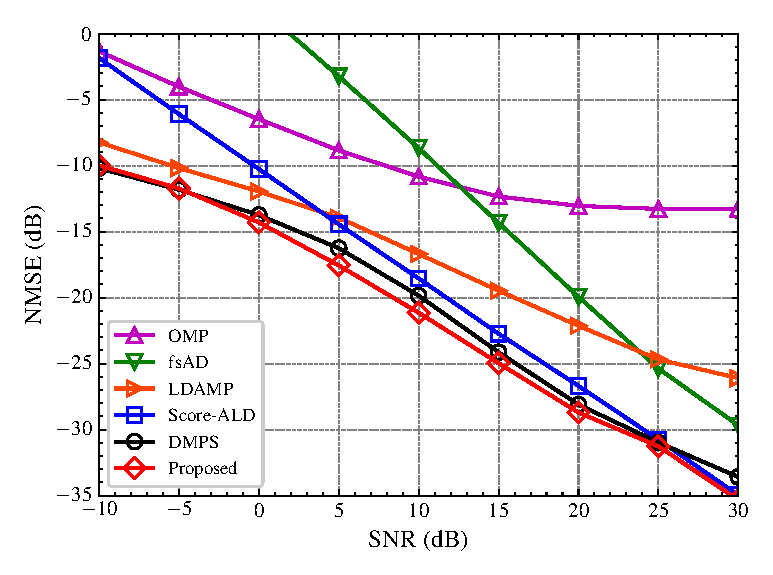
\includegraphics[width=0.48\textwidth]{images/results-1/CDL-D.eps}%
\label{fig:los-1}}
\\
\subfigure[NLOS]{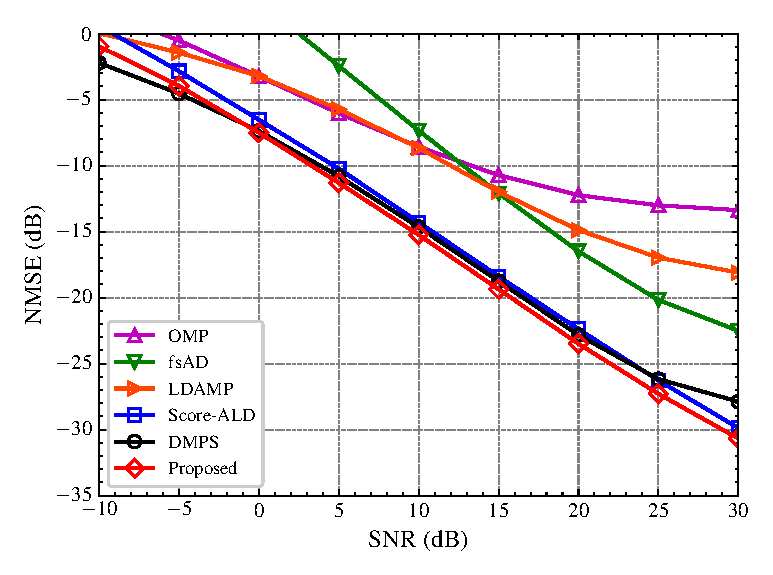
\includegraphics[width=0.48\textwidth]{images/results-1/CDL-B.eps}%
\label{fig:nlos-1}}
\caption{Channel estimation performance in terms of NMSE with $\rho$=0.6.}
\label{fig_sim_1}
\end{figure}

In Fig.~\ref{fig_sim_2}, robustness of the DM-based approaches was evaluated under the low pilot density. Specifically, at a pilot density of 0.3 in the LOS environment, it was confirmed that the proposed method outperforms the DMPS and Score-ALD by about 6 dB and 4 dB, respectively. Furthermore, the performance gap widens in the NLOS environment to about 12dB and 5dB compared to the DMPS and Score-ALD, respectively. Therefore, it was demonstrated that the robustness of the proposed method is attributable to a fundamental difference in the likelihood score approximation. While both DMPS and Score-ALD approximate the mean and covariance based on heuristic methods, the proposed method approximates them based on the moment matching principle and Tweedie's formula with the DM-based prior.

\begin{figure}[!t]
\subfigure[LOS]{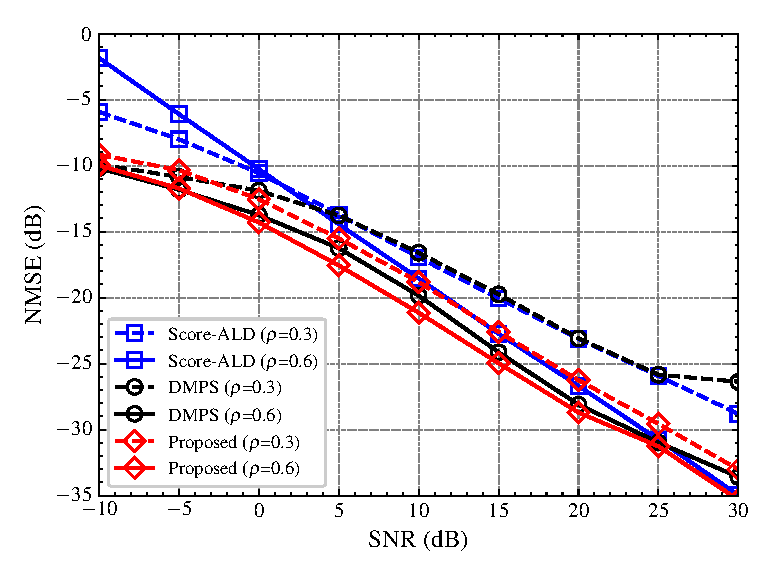
\includegraphics[width=0.48\textwidth]{images/results-2/CDL-D.eps}%
\label{fig:los-2}}
\\
\subfigure[NLOS]{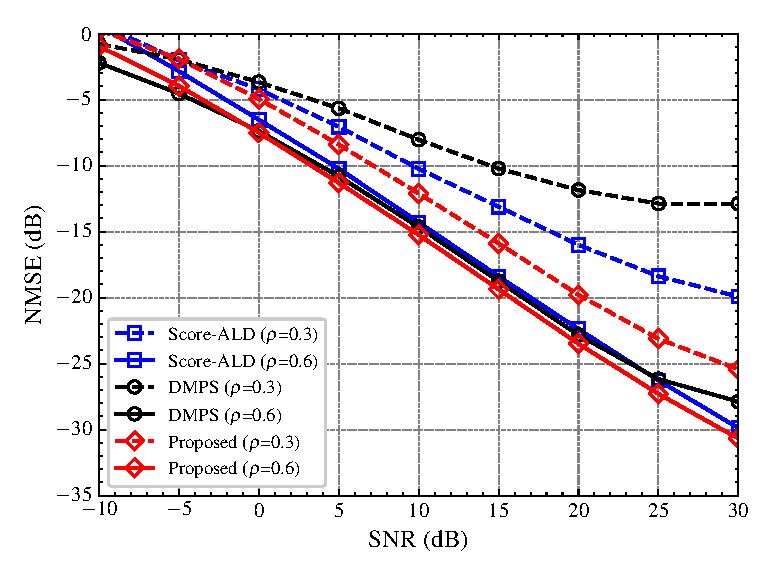
\includegraphics[width=0.48\textwidth]{images/results-2/CDL-B.eps}%
\label{fig:nlos-2}}
\caption{Robustness to pilot density in LOS and NLOS channels.}
\label{fig_sim_2}
\end{figure}

In order to verify the computational efficiency of the proposed method for deployments of practical wireless communication, we evaluated its floating-point operations (FLOPs), neural function evaluations (NFEs), and inference latency. The proposed method offers significant advantages in computational efficiency, as detailed in Table~\ref{tab:table1}, in terms of FLOPs, NFEs, and inference latency. The inference FLOPs were calculated by multiplying the FLOPs per function evaluation by the NFEs. The inference latency was measured in the condition of a batch size of 100 and pilot density of 0.6, averaged over 10 independent runs. The proposed method achieved about 65 times faster inference latency compared to Score-ALD. In comparison with DMPS, the proposed method achieved comparable latency while outperforming it in terms of FLOPs and NFEs. Consequently, it is shown that the proposed method can be a more accurate and efficient solution by providing a better trade-off between estimation accuracy and inference latency than the baselines.

\begin{table}[!t]
\centering
\renewcommand{\arraystretch}{1.1} 
\caption{Computational complexity for DM-based channel estimation methods in terms of FLOPs, NFEs, and latency}
\label{tab:table1}
\begin{tabular}{M{0.20\columnwidth}|M{0.21\columnwidth}|M{0.20\columnwidth}|M{0.20\columnwidth}}
\hline
\textbf{Method} & \textbf{FLOPs} & \textbf{NFEs} & \textbf{Latency (s)} \\
\hline
Score-ALD\cite{arvinteMIMOChannelEstimation2023} & \(1.028 \times 10^{12}\) & 6933 & 84.97 \\
\hline
% TODO: DMPS NFE가 변경되어 FLOPs 변경 필요
DMPS\cite{zhouGenerativeDiffusionModels2025} & \(2.449 \times 10^{10}\) & 130 & 1.27 \\
\hline
Proposed & \(4.899 \times 10^9\) & 20 & 1.29 \\
\hline
\end{tabular}
\end{table}

\section{Conclusion}

In this letter, a novel channel estimation method has been proposed to address the trade-off between accuracy, pilot overhead, and complexity in mmWave massive MIMO systems. Based on the moment matching principle and Tweedie's formula, the proposed method can perform accurate and efficient diffusion posterior sampling, achieving superior estimation accuracy compared to baselines with comparable computational complexity. From the simulation results, it is demonstrated that the proposed method has the potential to overcome a key bottleneck posed by high-dimensional channel. In future work, the extension of the proposed method to wideband and multi-user scenarios can be explored.

\bibliographystyle{IEEEtran}
% \bibliography{bib/IEEEabrv,bib/references}
\bibliography{bib/references}
\end{document}

